% experiments-draft-v1.tex (2026-11-10) -- the experiments section as a standalone draft for Yao.
% Every number is taken from a results file in the repository (named in comments). TBD marks the few cells still to be filled.
% Vocabulary follows paper/terminology-2026-11-10.md: BudgetMesh, MeshSplatting, the price lambda, rate-aware growth / collapse,
% the size controller, byte probe, target size, file size, the FP32 model, simplification after training, training with a vertex cap.
\documentclass[10pt]{article}
\usepackage[margin=1in]{geometry}
\usepackage{booktabs,multirow,graphicx,amsmath,xcolor,caption,subcaption,float,tabularx,array}
\usepackage[hidelinks]{hyperref}
\newcommand{\tbd}[1]{\textcolor{red}{[TBD: #1]}}
\newcommand{\MS}{MeshSplatting}
\newcommand{\BM}{BudgetMesh}
\title{\BM{}: experiments section, draft v1 for discussion}
\author{Devon Ren}
\date{November 10, 2026}
\begin{document}
\maketitle

\noindent\textbf{How to read this draft.} Each subsection is one claim, one table or figure, and the reviewer question it answers. Main-text items are marked [main]; items marked [appendix] are listed in Section~\ref{sec:appendix} with the same numbering. Numbers are final unless marked TBD. Figures are specified, not yet drawn; their captions are written so that the figure can be made to match.

%==================================================================
\section{Experimental setup}
\textbf{Datasets.} Mip-NeRF~360 (9 scenes: room, kitchen, counter, bonsai indoor; garden, bicycle, stump, flowers, treehill outdoor), Tanks and Temples (T\&T; truck, train), NeRF-Synthetic (8 objects), and Deep Blending (drjohnson, playroom). Deep Blending was not used while developing the method: every number on it comes from a single run with the settings fixed on the other datasets.

\textbf{Protocol.} \MS{} training is unchanged (30k iterations, its own schedule); images\_2 for indoor scenes, images\_4 for outdoor, the standard test split (every 8th view), black background for NeRF-Synthetic. Quality is PSNR/SSIM/LPIPS of the \emph{decoded file} rendered at the renderer's supersampling; all sizes are bytes of the single delivered file. The \emph{FP32 model} is the trained \MS{} mesh in 32-bit floats; its size and PSNR per scene are the reference for compression ratios and quality loss. ``At the same vertex count'' means after \MS{}'s final cleaning.

\textbf{Settings.} One configuration for all scenes: appearance dictionary $4096+256$, per-scene position grid (14--18 bits by scene extent), 7-bit DC colour; size controller with a growth aim of $1.25\times$ the target (Mip-NeRF~360, T\&T, Deep Blending) and $1.1\times$ (NeRF-Synthetic); collapse rounds every 500 iterations from 12.5k to 19.5k.

%==================================================================
\section{A trained mesh cannot be simplified afterwards [main]}
\label{sec:e1}
\textbf{Claim.} Reducing a trained \MS{} mesh to fewer vertices (collapse edges, then fine-tune) loses far more quality than training a mesh of that vertex count from the start. This is the reason the file size must be decided during training.

\begin{table}[H]\centering\small
\caption{Training with a vertex cap vs.\ simplification after training, at the same vertex count, three budgets per scene (the vertex counts of the 32$\times$/73$\times$/150$\times$ operating points). PSNR gain of the trained mesh over the simplified one, after our codec. Source: g0-refresh-analysis-2026-11-09.md, batch21-analysis-2026-11-10.md.}
\label{tab:e1}
\resizebox{\linewidth}{!}{\begin{tabular}{lrrrrr}
\toprule
Dataset & pairs & mean gain (dB) & range (dB) & trained better & gain at largest / mid / smallest budget \\
\midrule
Mip-NeRF 360 + T\&T & 33 & $+2.45$ & $+0.01$ to $+6.02$ & 33 / 33 & $+0.89$ / $+2.24$ / $+4.23$ \\
Deep Blending & 6 & $+2.71$ & $+1.39$ to $+4.72$ & 6 / 6 & $+1.48$ / $+2.91$ / $+3.75$ \\
NeRF-Synthetic & 32 & $+1.27$ & $+0.03$ to $+4.32$ & 32 / 32 & $+0.58$ / $+0.67$ / $+1.43$ / $+2.41$ (four budgets) \\
\midrule
all & 71 & $+1.94$ & $+0.01$ to $+6.02$ & 71 / 71 & \\
\bottomrule
\end{tabular}}
\end{table}

\noindent\textbf{Why.} Every pixel is covered by exactly one opaque triangle; when vertices are removed from a trained mesh the optimizer does not re-place the survivors, and the simplified mesh keeps far fewer faces per vertex (room at 486k vertices: 1.09M faces trained vs 0.94M simplified; bonsai at 266k: 671k vs 362k). The gap grows as the budget shrinks. Figure~\ref{fig:g0} shows it on one view.

\noindent\textit{Reviewer question answered:} ``Why not decimate after training, as one does with meshes?''

%==================================================================
\section{Rate-aware growth is a more efficient representation [main]}
\label{sec:e2}
\textbf{Claim.} At the same vertex count, and before any entropy coding, a mesh grown with the rate-aware rule reaches higher PSNR than \MS{} trained with a vertex cap. After the codec the advantage carries over at the same file size.

\begin{table}[H]\centering\small
\caption{\BM{} (rate-aware growth) vs.\ \MS{} with a vertex cap. Left: same vertex count, FP32 meshes, no codec. Right: same file size after our codec (the capped mesh is encoded with the same codec). Source: no-codec-equal-vertices-2026-11-09.md, g0-refresh-analysis-2026-11-09.md, batch21-analysis-2026-11-10.md.}
\label{tab:e2}
\resizebox{\linewidth}{!}{\begin{tabular}{lrrrrrr}
\toprule
 & \multicolumn{3}{c}{same vertex count, no codec} & \multicolumn{3}{c}{same file size, after codec} \\
\cmidrule(lr){2-4}\cmidrule(lr){5-7}
Dataset & pairs & mean gain & \BM{} better & pairs & mean gain & \BM{} better \\
\midrule
Mip-NeRF 360 + T\&T & 25 & $+0.40$ dB & 23 / 25 & 33 & $+0.33$ dB & 29 / 33 \\
\quad indoor only & 12 & $+0.58$ dB & 12 / 12 & & & \\
Deep Blending & 6 & $+0.15$ dB & 5 / 6 & 6 & $+0.19$ dB & 5 / 6 \\
NeRF-Synthetic & 14 & $+0.18$ dB & 13 / 14 & 32 & $+0.14$ dB & 28 / 32 \\
\bottomrule
\end{tabular}}
\end{table}

\noindent The ``pairs'' on the left are the budget runs whose final vertex count is within $\pm15\%$ of the \BM{} mesh they are compared with. The two halves separate the growth rule from the codec: the gain exists before any compression, and the codec compresses both meshes equally well.

\noindent\textit{Reviewer question answered:} ``Is the gain from the growth rule or from the codec?''

%==================================================================
\section{Size as an input [main]}
\label{sec:e3}
\textbf{Claim.} Given a target size, \BM{} delivers a file within about 10\% of it, with the same quality per byte as a constant-price run, on all four datasets with one setting.

\begin{table}[H]\centering\small
\caption{Size error and quality of \BM{} per dataset and target. Size error $=$ (file size $-$ target)$/$target; mean and range over scenes. $\Delta$PSNR is against the FP32 model. Rows at the capacity limit (the scene has no triangle left worth splitting; the price reaches its floor) are counted separately. Source: adapt-v9b sweep analysis, batch21-analysis-2026-11-10.md, budgetmesh-rd-table-2026-11-10.md.}
\label{tab:e3}
\resizebox{\linewidth}{!}{\begin{tabular}{llrrrrr}
\toprule
Dataset & target & scenes & mean file size & size error mean & size error range & $\Delta$PSNR vs FP32 \\
\midrule
\multirow{5}{*}{Mip-NeRF 360 + T\&T} & 5 MB & 11 & 5.0 MB & $+0.6\%$ & $-4.8$ to $+9.2\%$ & $-1.3$ dB \\
 & 7.5 MB & 11 & 7.6 MB & $+1.0\%$ & $-4.6$ to $+9.3\%$ & $-0.9$ dB \\
 & 10 MB & 11 & 10.2 MB & $+2.0\%$ & $-4.7$ to $+13.5\%$ & $-0.6$ dB \\
 & 15 MB & 11 & 15.2 MB & $+1.0\%$ & $-5.4$ to $+11.4\%$ & $-0.4$ dB \\
 & 20 MB & 11 & 19.9 MB & $-0.5\%$ & $-6.6$ to $+10.0\%$ & $-0.25$ dB \\
\midrule
\multirow{3}{*}{Deep Blending} & 5 MB & 2 & 5.4 MB & $+7.9\%$ & $+4.7$ to $+11.1\%$ & $-1.34$ dB \\
 & 10 MB & 2 & 11.0 MB & $+10.2\%$ & $+8.3$ to $+12.0\%$ & $-0.69$ dB \\
 & 20 MB & 2 & 21.3 MB & $+6.7\%$ & $+3.6$ to $+9.7\%$ & $-0.28$ dB \\
\midrule
\multirow{5}{*}{NeRF-Synthetic$^\dagger$} & 1.5 MB & 8 & 1.56 MB & $+4.0\%$ & $+1.0$ to $+9.0\%$ & $-0.88$ dB \\
 & 2.5 MB & 7 (+1 cap.) & 2.56 MB & $+2.6\%$ & $-6.6$ to $+9.2\%$ & $-0.30$ dB \\
 & 3 MB & 5 (+2 cap.; materials run missing) & 3.05 MB & $+1.8\%$ & $-4.6$ to $+7.0\%$ & $-0.13$ dB \\
 & 4 MB & 6 (+2 cap.) & 3.9 MB & $-2.9\%$ & $-10.3$ to $+3.4\%$ & $-0.13$ dB \\
 & 6 MB & 2 (+6 cap.) & 5.7 MB & $-5.0\%$ & $-11.5$ to $+1.5\%$ & $+0.10$ dB \\
\midrule
\multicolumn{7}{l}{$^\dagger$NeRF-Synthetic reference = the fine-tuned FP32 original (val-selected checkpoint), so small positive values occur.}\\
\multicolumn{7}{l}{Overall: 89 rows not at the capacity limit, 83 within $\pm10\%$; quality at the same file size vs.\ a constant-price run: $-0.05$ dB mean (Table~\ref{tab:e7}).}\\
\bottomrule
\end{tabular}}
\end{table}

\begin{figure}[H]\centering
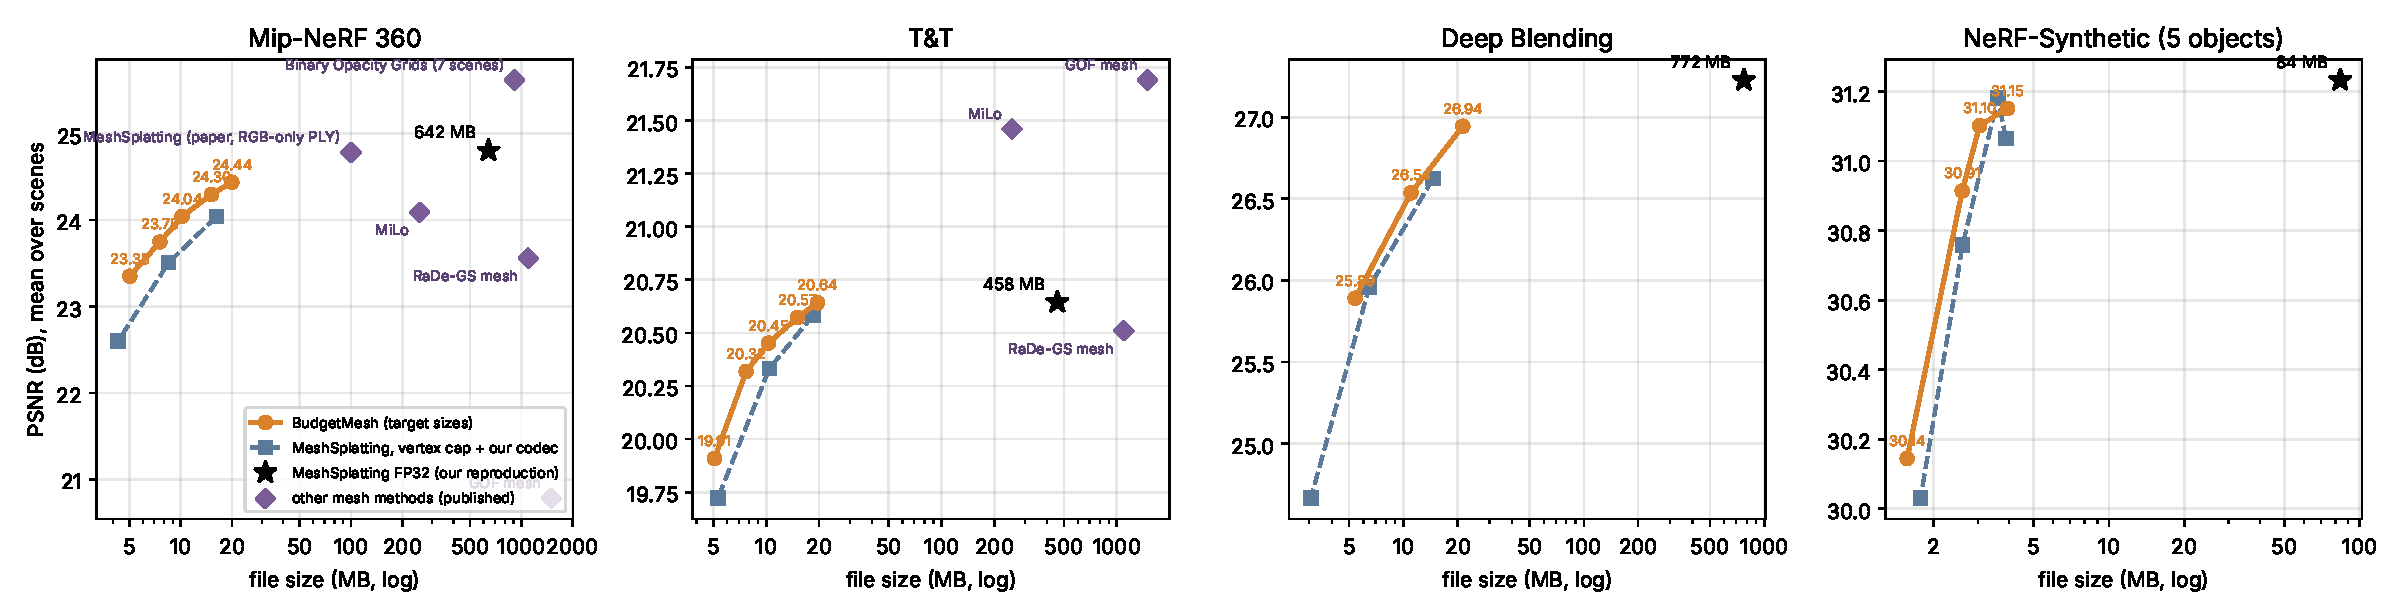
\includegraphics[width=\linewidth]{figures/fig_rd_per_dataset.pdf}
\caption{Rate--distortion of \BM{} per dataset: mean PSNR vs.\ mean file size over the dataset's scenes at each target (orange), \MS{} trained with a vertex cap and encoded with the same codec (blue), and the FP32 model (star). NeRF-Synthetic uses the five objects that are below their capacity limit at every target. Per-scene curves in the appendix.}
\label{fig:rd}
\end{figure}

\noindent\textbf{Reading the table.} Indoor scenes land 5--12\% above the target: after the growth phase ends, the set of visible faces keeps growing while \MS{} raises its opacity floor, and the collapse rounds can only remove so much per round. Outdoor scenes at 20 MB land up to 7\% below: the last growth round admits fewer splits than planned and nothing can add vertices afterwards. Both are discussed as limitations. On NeRF-Synthetic several objects cannot fill 4--6 MB at all (the price falls to its floor from the first rounds); the controller reports this rather than forcing splits.

\noindent\textit{Reviewer questions answered:} ``Does controlling the size cost quality?'' (no: $-0.05$ dB) and ``Does it generalise?'' (Deep Blending, untouched settings).

%==================================================================
\section{Compression results [main]}
\label{sec:e4}
\begin{table}[H]\centering\small
\caption{Compression against the FP32 model, means over scenes; per scene in the appendix. Source: budgetmesh-rd-table-2026-11-10.md.}
\label{tab:e4}
\begin{tabular}{lrrrr}
\toprule
Target & scenes & mean ratio & mean $\Delta$PSNR & $\Delta$PSNR range \\
\midrule
20 MB & 13 & 32$\times$ & $-0.30$ & $-0.72$ to $+0.16$ \\
15 MB & 11 & 40$\times$ & $-0.43$ & $-0.93$ to $+0.05$ \\
10 MB & 13 & 62$\times$ & $-0.66$ & $-1.31$ to $+0.07$ \\
7.5 MB & 11 & 81$\times$ & $-0.92$ & $-2.07$ to $-0.15$ \\
5 MB & 13 & 125$\times$ & $-1.32$ & $-2.47$ to $-0.29$ \\
\bottomrule
\end{tabular}
\end{table}
\noindent The decoder is a standalone program (no access to training data) that reconstructs a standard indexed mesh in 2.3--6.4 s on one CPU core (0.4--1.1M vertices); the decoded mesh renders with an ordinary vertex shader at 145--350 fps on a phone (iPhone 17 Pro, full capture resolution; table2-deployability-v1).

\section{Against generic mesh codecs [main, one table; full data appendix]}
\label{sec:e5}
\textbf{Claim.} Standard mesh codecs cannot reach our sizes while keeping view-dependent appearance; the only generic routes near our size drop it and still produce larger files.

\begin{table}[H]\centering\small
\caption{The same FP32 mesh through generic codecs vs.\ ours (our level-1.0 delivery of that mesh). Ratios are generic file size divided by ours, over 11 Mip-NeRF~360 / T\&T scenes (MPEG: 10). Source: generic-codecs-all-scenes-2026-11-10.md.}
\label{tab:e5}
\resizebox{\linewidth}{!}{\begin{tabular}{lrrl}
\toprule
Route & size vs.\ ours (Deep Blending) & $\Delta$PSNR vs FP32 & keeps view dependence \\
\midrule
Draco, positions + faces + 8-bit SH & 12--18$\times$, mean 15$\times$ (16$\times$) & $-0.02$ to $-0.2$ dB & yes \\
MPEG SC3DMC/TFAN, positions + faces + 8-bit SH & 3.1--4.2$\times$, mean 3.7$\times$ (3.3$\times$) & $-0.02$ to $-0.2$ dB & yes \\
Quantised PLY + zstd-19 & $\approx$5--7$\times$ & $-0.02$ to $-0.2$ dB & yes \\
Draco, positions + faces + 8-bit RGB & 1.8--2.4$\times$ & $-0.7$ to $-4.4$ dB & no \\
Baked $4096^2$ texture + Draco geometry & $\approx$2.5--3.5$\times$ & $-0.7$ to $-4.4$ dB & no \\
Ours (level 1.0) & 1$\times$ & $-0.1$ to $-0.8$ dB & yes \\
\bottomrule
\end{tabular}}
\end{table}
\noindent\textbf{Caveat stated in the text.} The generic rows are near-lossless and ours loses 0.1--0.8 dB at this point, so this is ``bytes each codec needs for essentially the same mesh'', not an RD curve; the RD comparison with 3DGS-class codecs is in the appendix (Section~\ref{sec:appendix}, A5) and shows the representation gap honestly.

%==================================================================
\section{Where the bytes go, and what is redundant [main, short]}
\label{sec:e6}
\begin{figure}[H]\centering
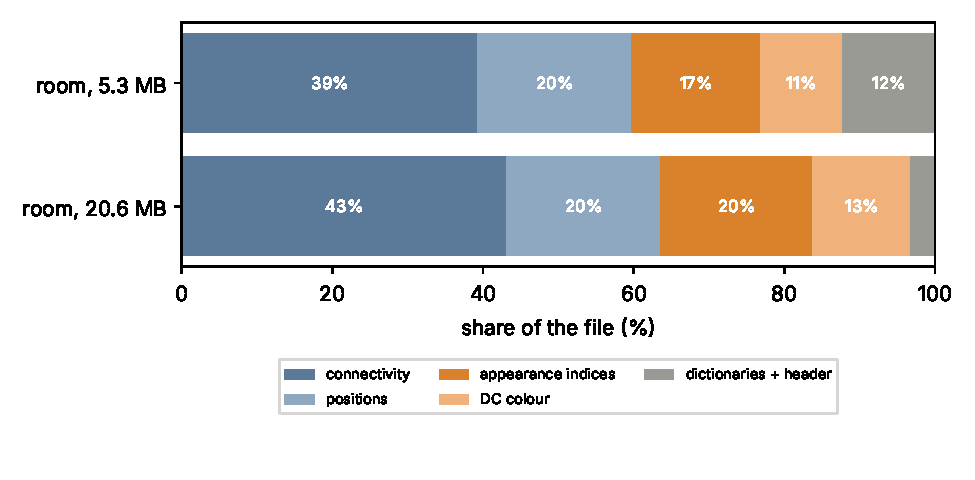
\includegraphics[width=0.75\linewidth]{figures/fig_bytes_per_stream.pdf}
\caption{Bytes per stream. Connectivity is 39--43\% of the file and lossless; positions 20\%; appearance indices 17--20\%; DC colour 11--13\%; the dictionaries are a fixed 0.65 MB, 3\% of a 20 MB file and 12\% of a 5 MB one.}
\label{fig:bytes}
\end{figure}
\noindent Two findings, each one sentence in the text with its number: (i) \emph{appearance sharing carries the loss}: at the top rate, 8-bit instead of 7-bit DC colour recovers only 0.04--0.08 dB of the 0.4--0.6 dB loss on indoor scenes; (ii) \emph{dictionary size should follow vertex count}: the fixed $4096+256$ is within 0.16 dB of the best dictionary at every point on Mip-NeRF~360, T\&T and Deep Blending, but on the smallest objects (mic, ficus) a 1024-entry dictionary at a lower price is $+0.5$--$0.6$ dB at the same file size. Full sweep in the appendix.

%==================================================================
\section{Ablations [main, one table]}
\label{sec:e7}
Table~\ref{tab:e7} removes one part of the training rule at a time and reports what happens to the size and to the quality at the same file size. The constant-price row is the only place where constant-$\lambda$ runs appear in the paper.
\begin{table}[H]\centering\small
\caption{What each part of the training rule contributes. Source: adapt-v9b sweep analysis (constant price), adapt-v7b sweep (prices from constants), rd-ctrl-v1 (matched count), v6 Blender tests (collapse off).}
\label{tab:e7}
\begin{tabularx}{\linewidth}{>{\raggedright\arraybackslash}p{4.2cm}XX}
\toprule
Variant & size & quality at the same file size \\
\midrule
full \BM{} & within $\pm10\%$ on 83/89 & reference \\
constant price (controller off) & unpredictable: one price lands at 15--100\% of the dense vertex count depending on the scene & $+0.05$ dB (33 rows) \\
prices from fixed constants instead of the byte probe & mean 0.83$\times$ target, 8/33 within $\pm10\%$ & $-0.05$ dB \\
no in-training collapse & lands at the growth aim: $+25\%$ by construction (nothing removes bytes after growth) & $-0.3$ / $-0.5$ dB (lego / chair at 4 MB, v6 tests) \\
\MS{}'s own split selection at the same split count & same & $-0.12$ dB (room) \tbd{one more scene optional} \\
\bottomrule
\end{tabularx}
\end{table}

%==================================================================
\section{Qualitative results [main]}
\label{sec:e8}
Figure~\ref{fig:qual} shows decoded files at the three main targets next to the ground truth and the FP32 model, with an enlarged crop and the error map per column; Figure~\ref{fig:g0} shows the same vertex count reached three ways (the experiment of Section~\ref{sec:e1}) on one view.
\begin{figure}[H]\centering
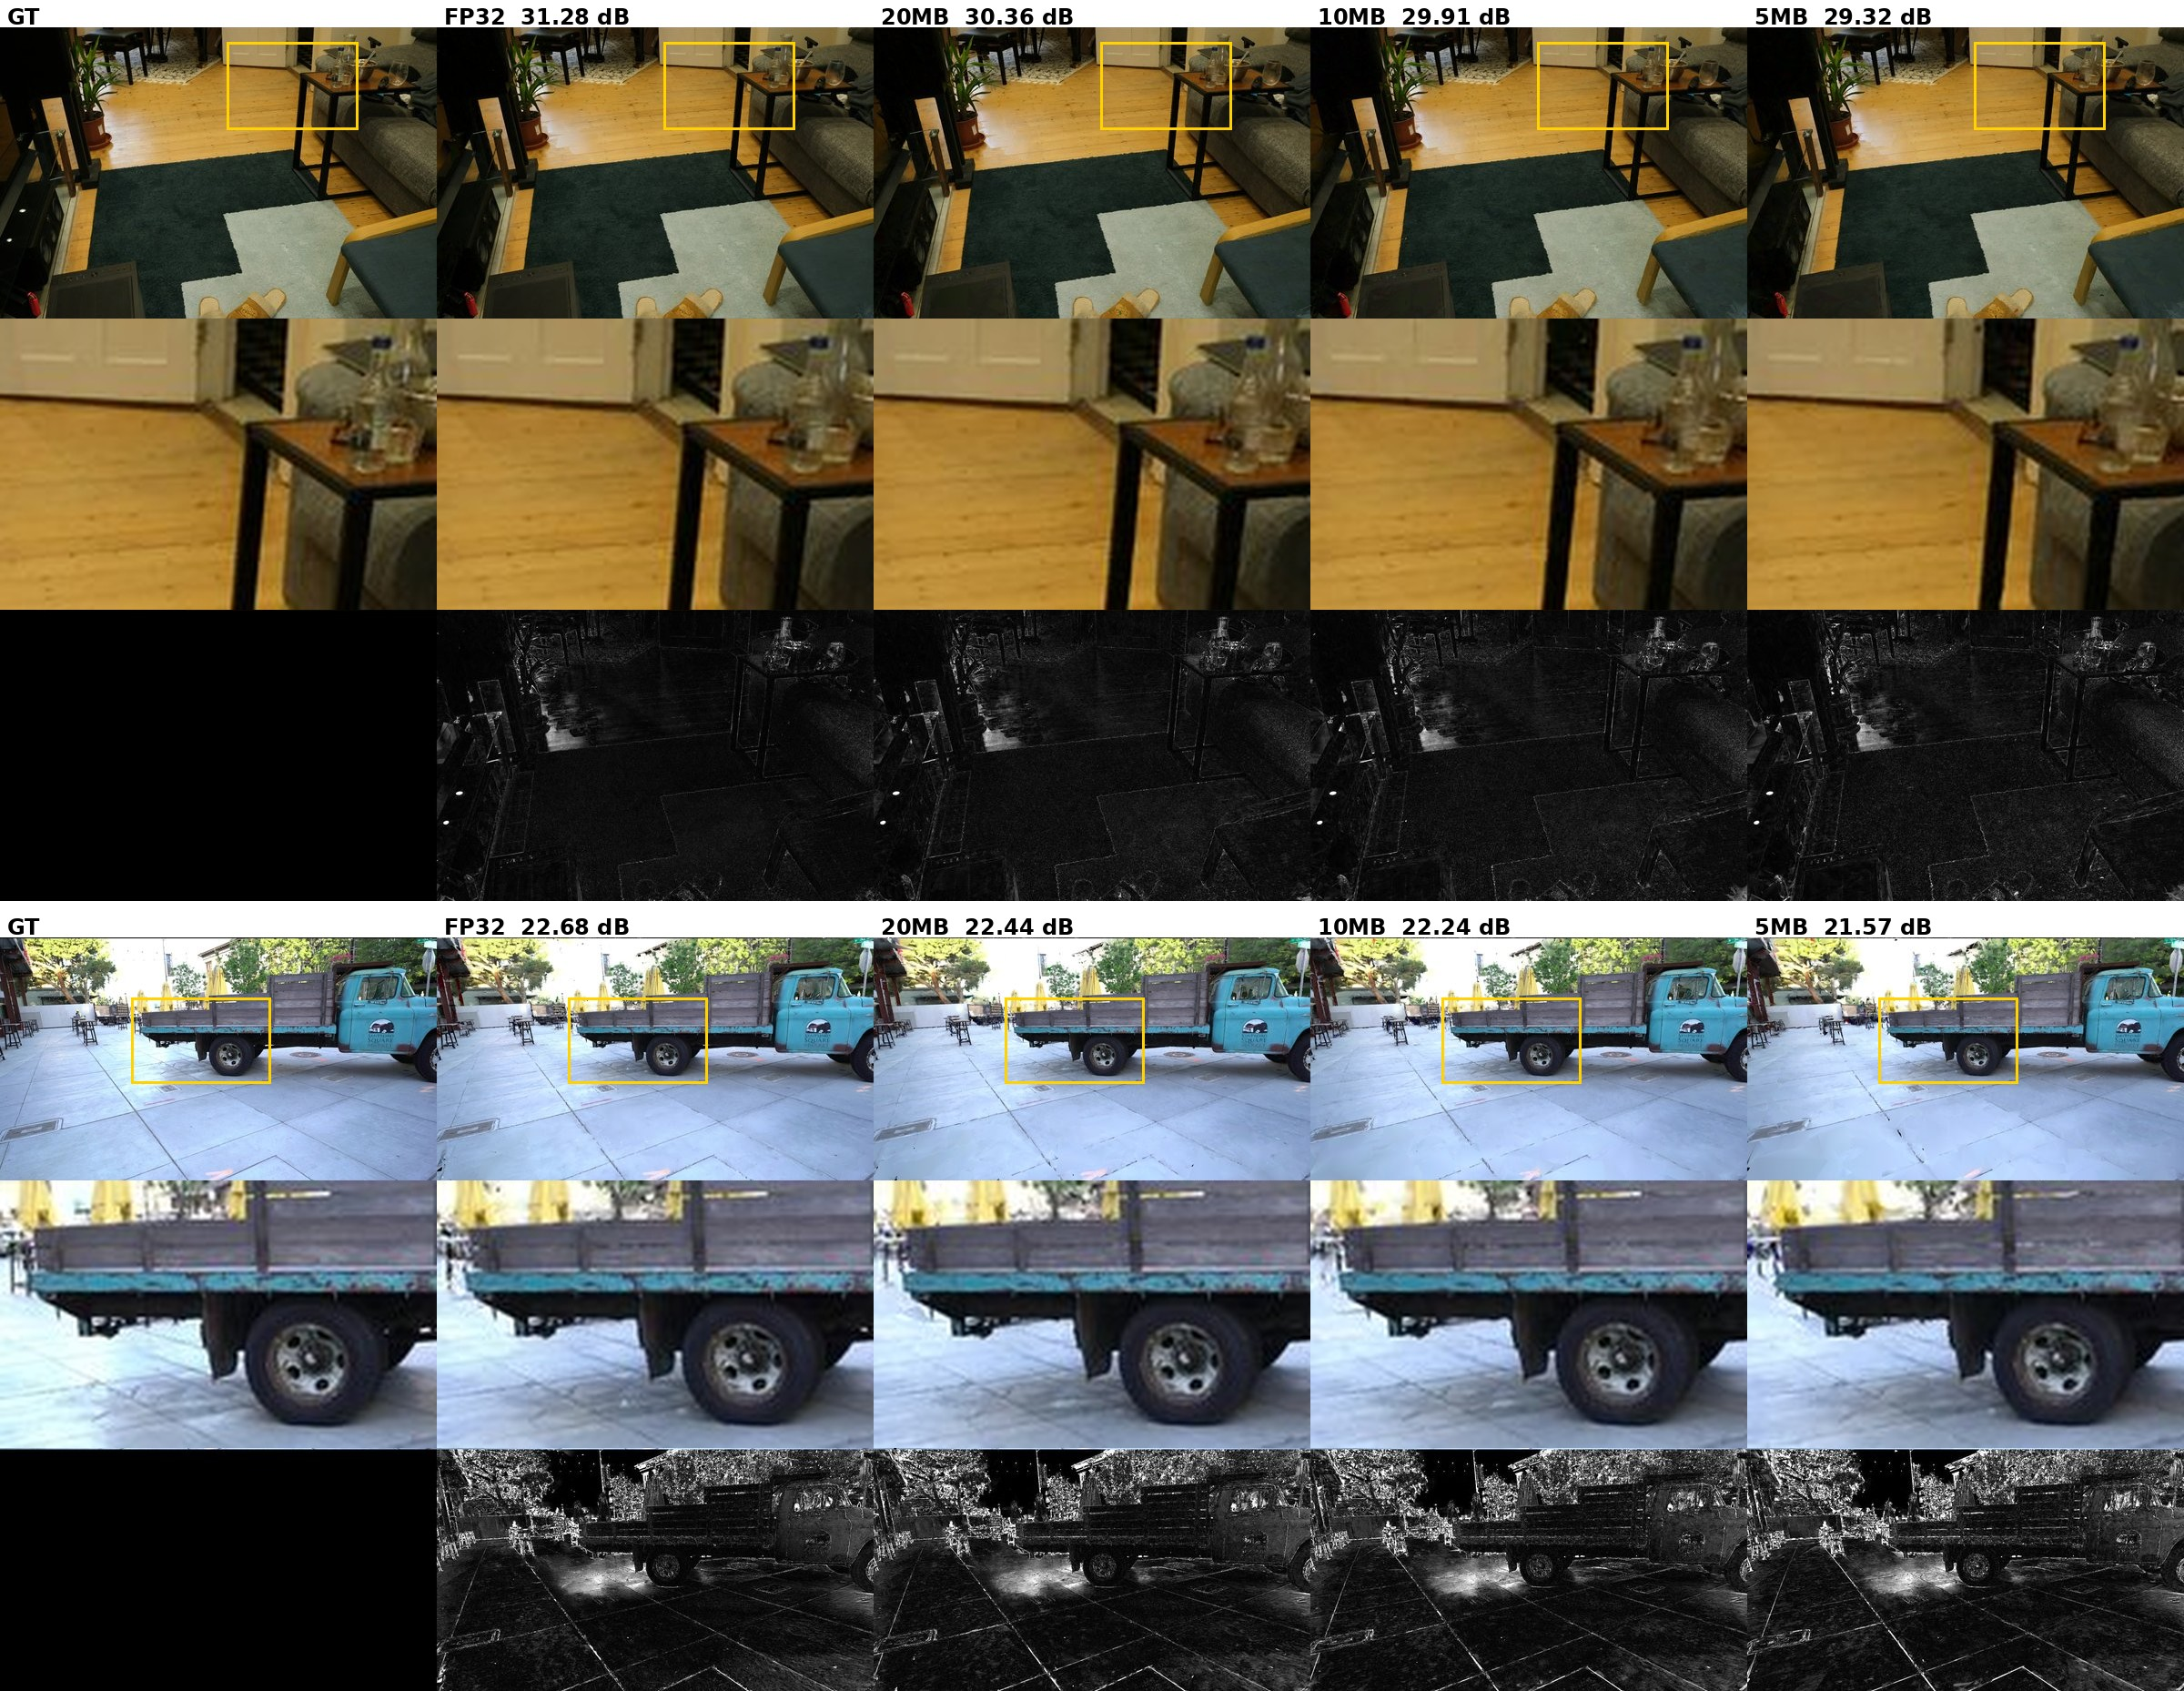
\includegraphics[width=\linewidth]{figures/fig_qualitative.jpg}
\caption{Decoded \BM{} files at three target sizes next to the ground truth and the FP32 model (room, truck). Per column: full view with its PSNR, the yellow-box crop enlarged, and the error map ($|$render $-$ GT$|\times4$). Draft version from quarter-resolution montages; the camera-ready crops will be cut from the full-resolution renders.}
\label{fig:qual}
\end{figure}
\begin{figure}[H]\centering
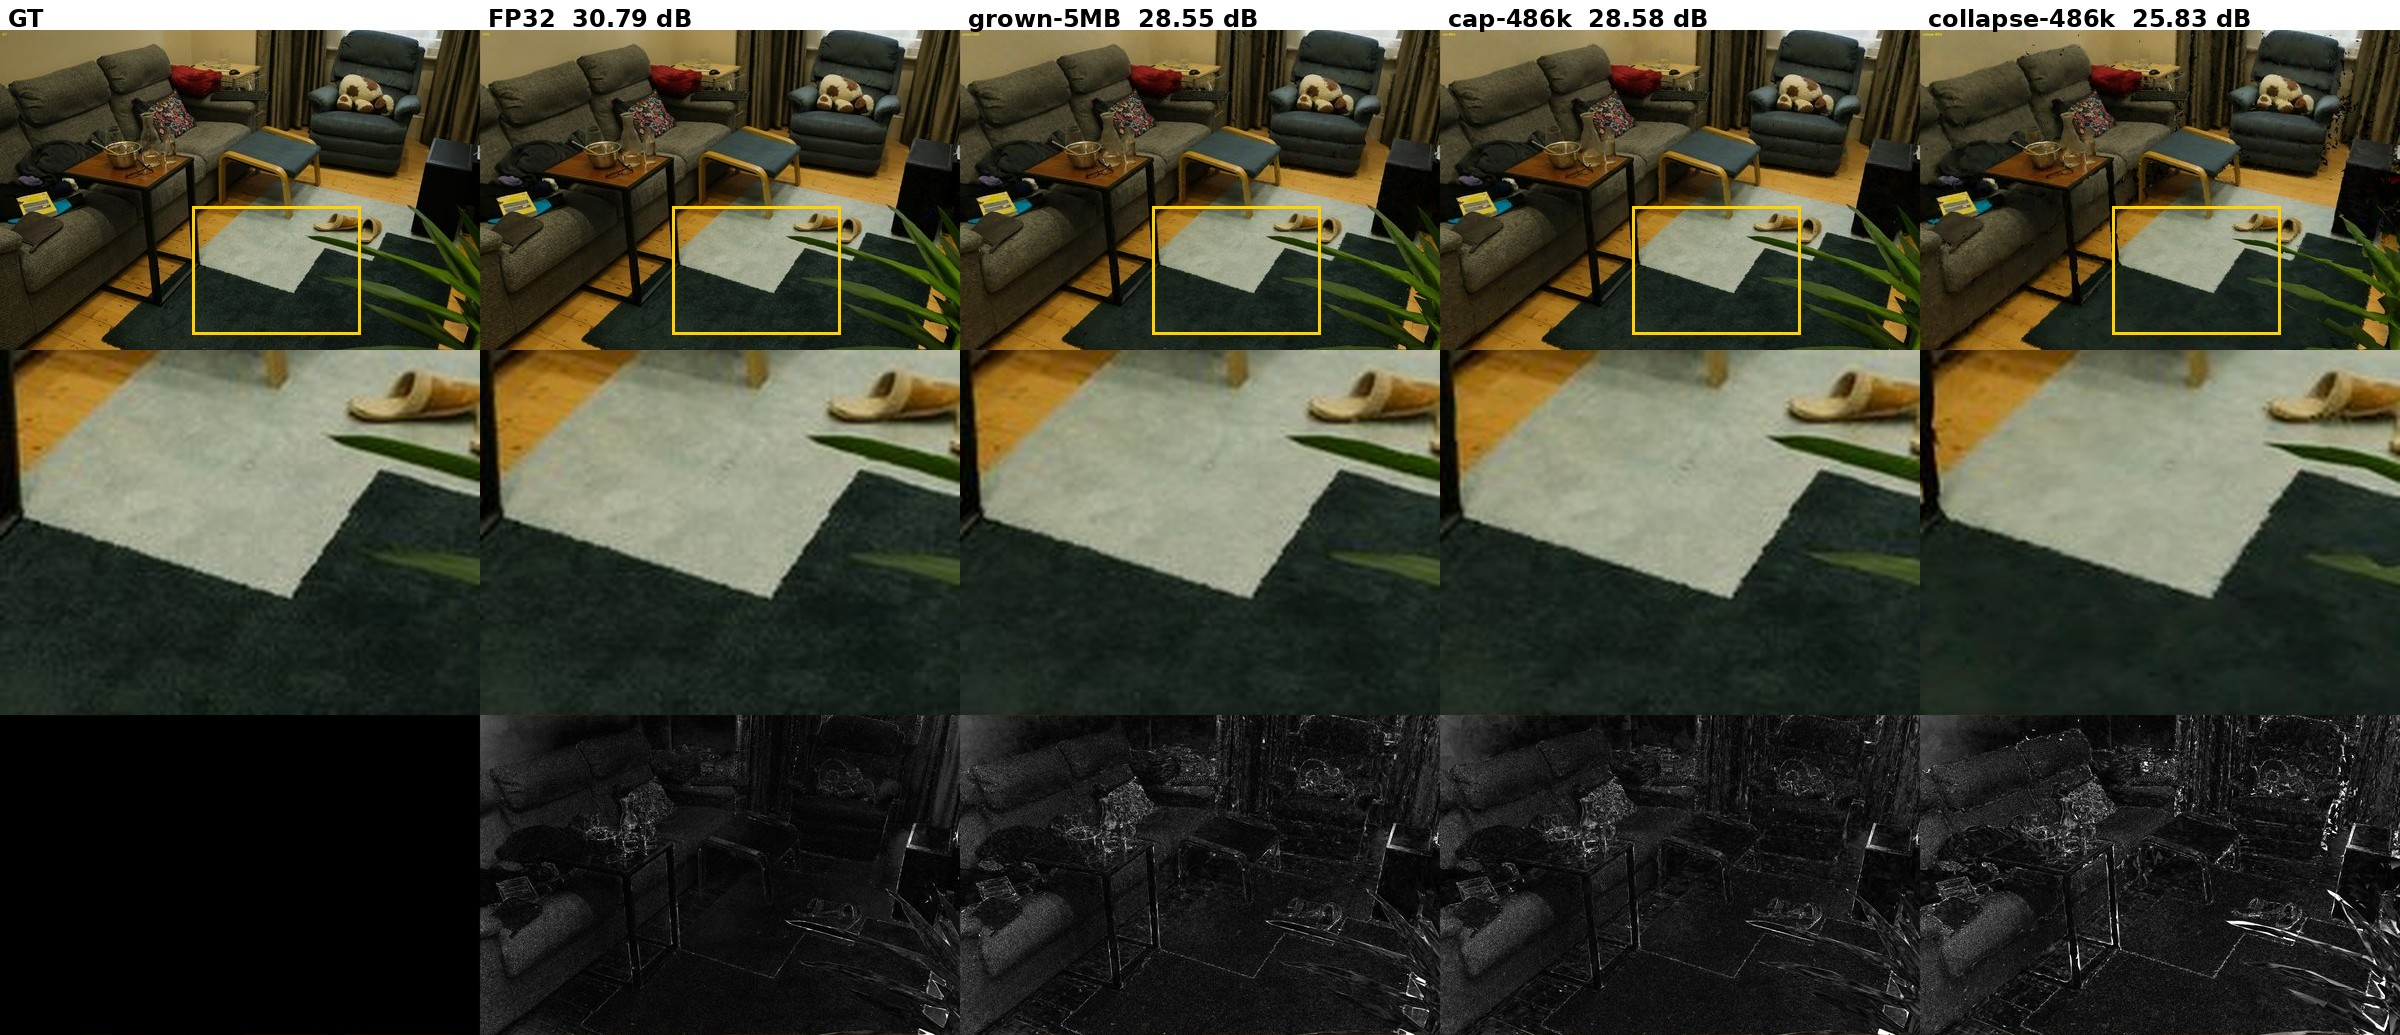
\includegraphics[width=\linewidth]{figures/fig_g0_triptych.jpg}
\caption{The same vertex count reached three ways. Simplification after training loses 3 dB on this view and shows holes and speckle; training to the budget does not.}
\label{fig:g0}
\end{figure}

%==================================================================
\section{Properties of the size controller [main, short]}
\label{sec:e9}
Two statements hold by construction. (1) The collapse rounds never move the file size below the target: each round removes at most the estimated excess and only while the estimate is above the target, so the size error from trimming is one-sided. (2) With $R$ rounds, a per-round cap of $c$ of the vertices and $b$ bytes freed per collapse, the trimming capacity is at most $R\,c\,V\,b$; the final overshoot is bounded by the excess at the first round minus this capacity, plus whatever the visible set grows after the last round. The growth plan re-spreads the remaining gap over the rounds left at every boundary, so a shortfall in one round is corrected in the next; only the last round's shortfall is not. Figure~\ref{fig:traces} shows the landing-estimate traces of all runs; Figure~\ref{fig:hist} the size error of every run by dataset and target.
\begin{figure}[H]\centering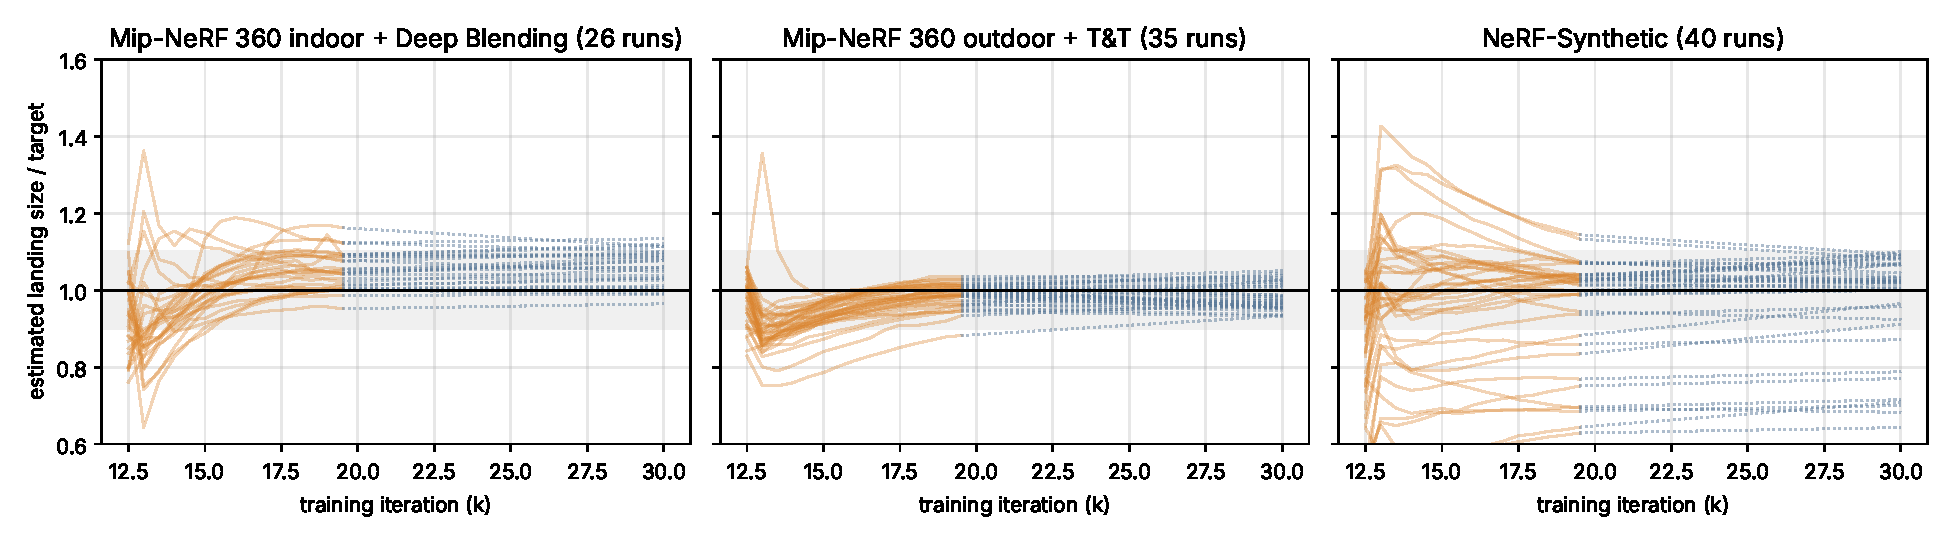
\includegraphics[width=\linewidth]{figures/fig_controller_traces.pdf}
\caption{Size controller traces for all 101 runs: the estimated landing size divided by the target at each collapse round (orange), continued as a dotted line to the delivered file. Grey band: $\pm10\%$. Indoor scenes start above the target (the growth aim) and are trimmed down; outdoor scenes start below and drift up as the visible set grows; the NeRF-Synthetic runs below 0.8 are objects at the capacity limit.}\label{fig:traces}\end{figure}
\begin{figure}[H]\centering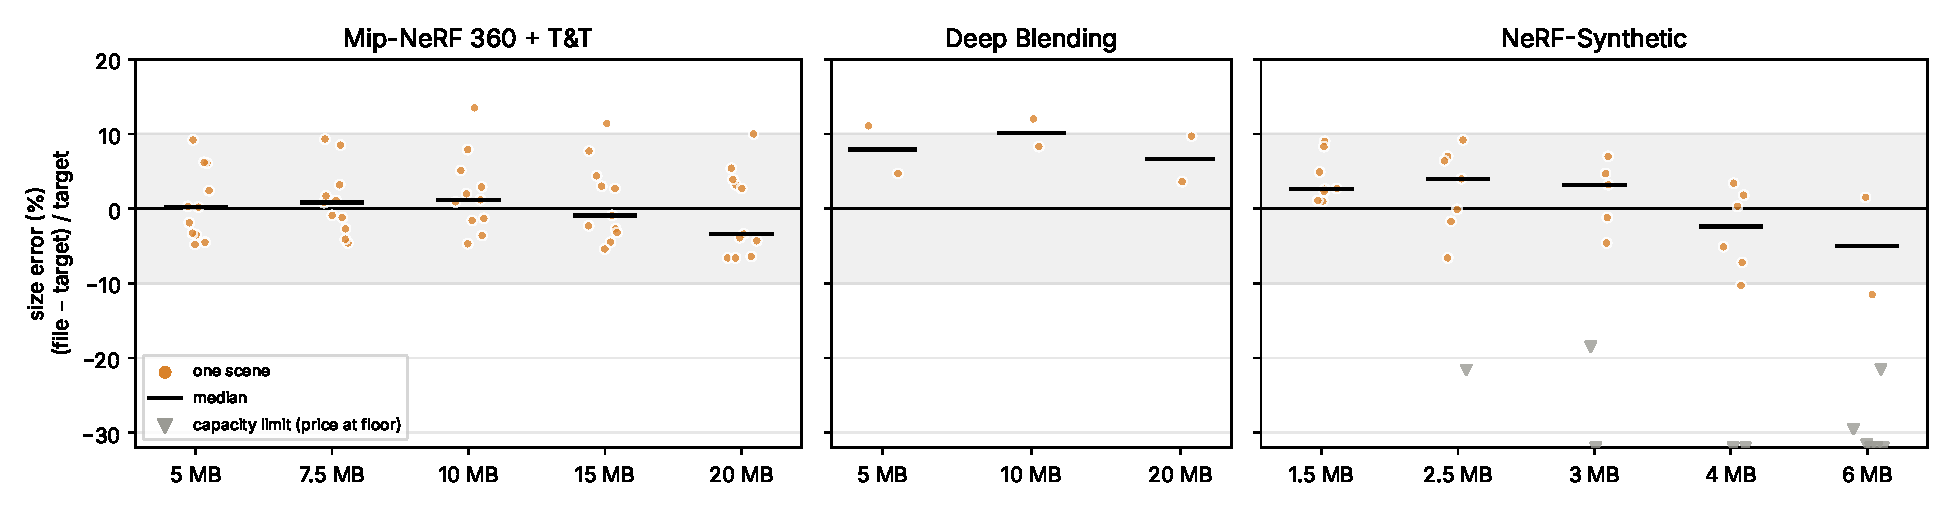
\includegraphics[width=\linewidth]{figures/fig_size_error_strip.pdf}
\caption{Size error of every run, one dot per scene, by dataset and target; black bar: median; grey band: $\pm10\%$. Grey triangles are objects at the capacity limit (the price reached its floor; the file cannot grow to the target).}\label{fig:hist}\end{figure}

%==================================================================
\section{Limitations}
The growth aim ($1.25\times$ / $1.1\times$) is one calibrated constant per capture class; it stands in for the growth of the visible-face set after the growth phase, which cannot be observed before \MS{} stitches the mesh. Indoor scenes land 5--12\% above the target; outdoor scenes at 20 MB up to 7\% below. Small objects cannot fill large targets (model capacity; reported, not hidden). Opaque meshes are about 3 dB below Gaussian-splat codecs at the same file size (A5); that gap is the representation's, and this paper is about what the mesh class can do per byte. The entropy coder is fixed, not learned.

%==================================================================
\section{Appendix items}
\label{sec:appendix}
\begin{description}
\item[A1] Controller traces: landing estimate vs.\ collapse round for all 89 runs (two panels, indoor / outdoor), target normalised to 1. Shows the gate opening, monotone descent, and the drift. \tbd{figure from rd\_log.jsonl}
\item[A2] Size-error histogram per dataset; aim factor 1.0 vs 1.25 on the same scenes (one-sided under-shoot becomes centred). Source: v7/v9b sweeps.
\item[A3] Per-scene tables for Sections~\ref{sec:e1}--\ref{sec:e4} (71 + 33 + 89 rows), including the capacity-limited NeRF-Synthetic rows.
\item[A4] Full generic-codec table (13 scenes, all routes, MB and PSNR).
\item[A5] Cross-representation figure (Figure~\ref{fig:cross}): \BM{}'s Mip-NeRF~360 curve with the published points of other mesh-output methods (MeshSplatting's own RGB-only file, MiLo, BakedSDF, Binary Opacity Grids, RaDe-GS and GOF meshes) and of 3DGS-class codecs (3DGS, Scaffold-GS, Compact3DGS, LightGaussian, RDO-Gaussian, HAC, HAC++, CompGS; HAC++ Table II). Honest reading: within the mesh class ours is the only entry below 100 MB and is 5--100$\times$ smaller than the others at comparable or better PSNR; against 3DGS codecs we are 3--4 dB lower at the same size, a gap already present between FP32 \MS{} (24.8) and 3DGS (27.5) on the same scenes, i.e.\ the representation's, not the codec's. Their output needs a splat renderer; ours is a standard mesh.
\begin{figure}[H]\centering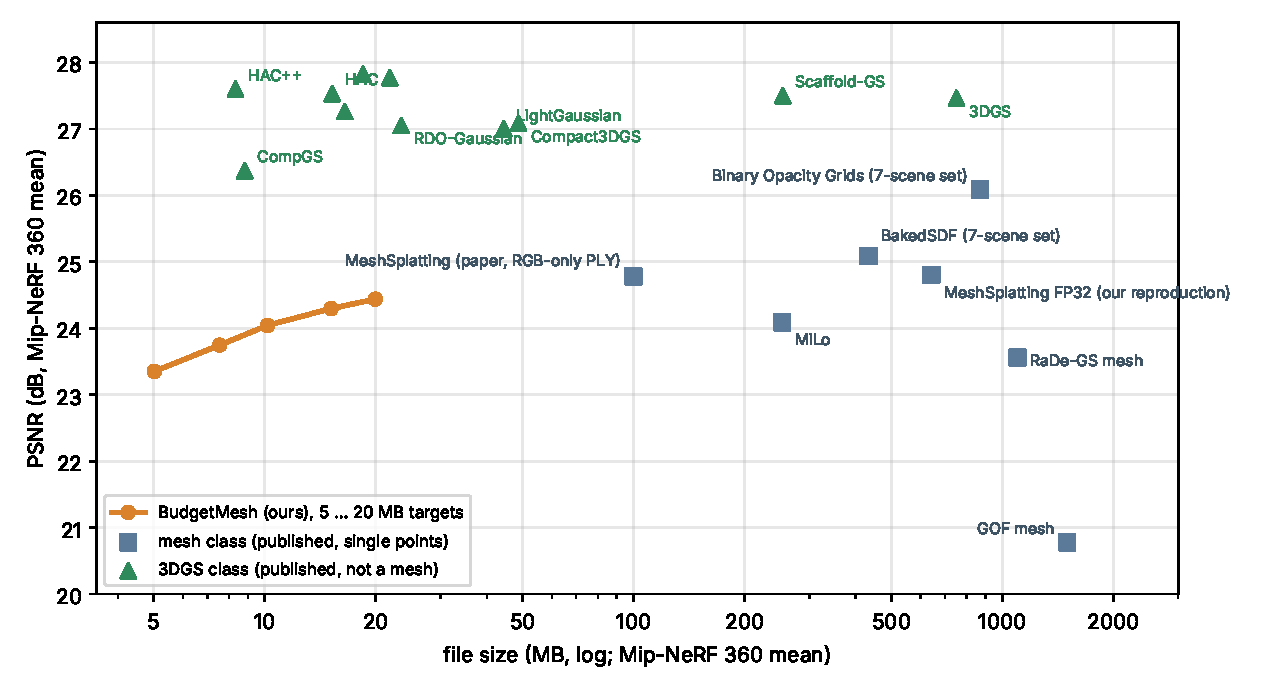
\includegraphics[width=0.85\linewidth]{figures/fig_cross_methods_mip360.pdf}
\caption{Mip-NeRF~360 means: \BM{} (curve) against published single points of mesh-output methods (squares) and 3DGS-class codecs (triangles). BakedSDF and Binary Opacity Grids report the 7-scene subset. Sizes are the methods' own reported asset sizes.}\label{fig:cross}\end{figure}
\item[A6] Dictionary $\times$ price sweep, all 21 scenes; DC 8-bit rows; the $K$-should-follow-$V$ observation with the mic/ficus numbers.
\item[A7] Byte-probe accuracy (probe / delivered 0.999--1.001 on 49 runs), per-run overhead (+8--15 min), the price schedule $\lambda$ per boundary for one scene.
\item[A8] Decoder audit: isolation test, stream list, file format.
\item[A9] Mesh statistics of delivered assets and the un-stacking measurement behind the aim factor.
\item[A10] Remaining qualitative rows (garden, Deep Blending, lego).
\end{description}

\end{document}
